\chapter{Common Errors in Supervised Modelling}

Here we shows some common errors with supervised learning. These errors are general---not limited to \mutation. Understanding them improves our understanding of supervised learning and might even influence our approach to data acquisition. We are going to simulate these errors as follows:

\begin{enumerate}
\item First, create a data set where classes should be impossible to predict.
\item Then, do some operations on the data.
\item Finally, observe that supervised learning found some way of discriminating the classes.
\end{enumerate}

Since data was prepared to be inseparable, any correlation between features in the data and the classes should be spurious correlations.

% LECTURE, prepare this as a slide so that students better understand the setting

\section{Predicting on the training data}

We will first create a data set with no correlation between spectra and their class variable. To do this, we open the ``Liver spectroscopy'' data set and shuffle the classes with \widget{Randomize} (set it to shuffle 100\%). \widget{Randomize} destroys any connection between features and the class variable. Therefore, supervised models should perform badly on this data set. More precisely, we would expect them to perform similarly to the majority classifier (that is a classifier that assigns a sample to a class which is in the majority in the training set). \textbf{Verify with cross-validation on the randomized and non-randomized data sets}.

Next, build a \widget{Tree} on the randomized data and look at predictions on the whole data set: \widget{Predictions}. The \widget{Tree} seems to perform almost perfectly. We know that classes were randomized, so there should be no correlations between spectra and the classes. How could a \widget{Tree} even model anything?

\begin{center}
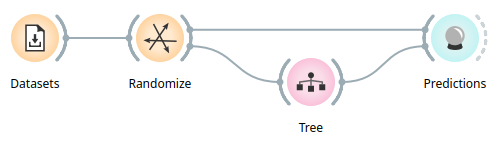
\includegraphics[scale=0.5]{predicting-training.png}
\end{center}

To answer the previous question, observe trees (with a \widget{Tree Viewer}) built on both randomized and non-randomized data. Notice that the tree on randomized data is much more complex. The tree can grow indefinitely and can, therefore, model any correlations, no matter how small these correlations are. Even random data will provide enough correlations for a tree model. Fortunately, correlations between spectra and classes in randomized data differ in each subset of data. Therefore, testing on separate test sets will allows us to discover if the model is overfitted.

Some methods are more prone to overfitting than others. It is harder to overfit with PLS or logistic regression than with classification trees. However, even PLS or logistic regression have a tendency to overfit. \textbf{Try and see the difference}. In addition, some models have parameters controlling model complexity. \textbf{Explore effects of parameters in the \widget{Tree} widget}.

We saw that we can build seemingly good models even on data where it should be impossible if we do not properly evaluate the models. Therefore, validate all models carefully.


\section{Separate preprocessing of data corresponding to different classes may introduce spurious correlations}

We will now create another dataset and classes that should be impossible to classify: we randomly split spectra it into two groups, and annotate each group with a different class value. For this numerical experiment, we will use the ``Hair section'' data set, which contains spectra on multiple hair sections organized as a spectral image. For simplicity, select one section in the \widget{HyperSpectra} widget (use polygonal selection).  Then, split the data randomly into two halves with the \widget{Data Sampler} widget. Join the two halves together with \widget{Concatenate} (set it to add a class column depending on the source). Now, we have a data set that is hard to classify since the classes are random. \textbf{Perform cross-validation and report the scores}.

\begin{center}
\end{center}
\begin{figure*}[h]
\centering
\vspace{-0.5cm}
\infinitewidthbox{
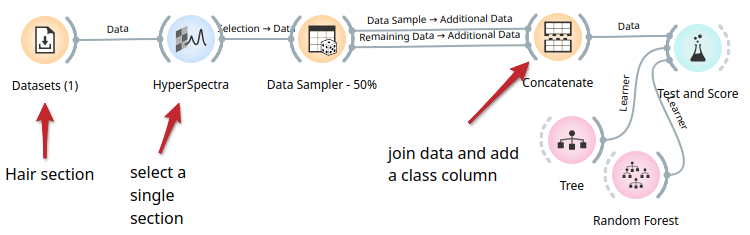
\includegraphics[scale=0.5]{different-classes-hair-start.png}
  }
\caption{Learning methods perform badly here. AUC should be around 0.5.}
\end{figure*}

Next, let us introduce separate preprocessing for each of the classes. For each class, we will subtract a different background spectrum. Select one background spectrum per group (two \widget{HyperSpectra} widgets) and send them as references into corresponding \widget{Preprocess Spectra} widgets. Preprocess with Spectrum subtraction with weight set to 1. Notice that the preprocessing effect is very slight. After concatenating, perform cross-validation. \textbf{Report the scores. How large was the effect of only slightly different preprocessing?}

\begin{center}
\end{center}
\begin{figure*}[h]
\centering
\vspace{-0.5cm}
\infinitewidthbox{
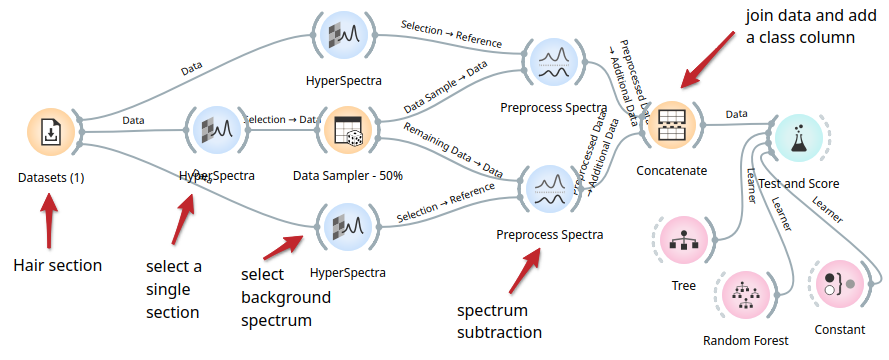
\includegraphics[scale=0.5]{different-classes-hair.png}
  }
\caption{Even slightly different preprocessing allows random classes to separate easily, if preprocessing was done for each class separately.}
\end{figure*}

What happens with other types of preprocessing? \textbf{Try other preprocessing methods. Which methods produce separable data and which do not? What do they have in common?}

We saw that even slight differences in preprocessing create a significant fake signal.
A similar 'fake effect' may happen as well when you measure samples of different classes on different days. Some physical conditions, e.g. in the instrument, may introduce a systematic error, e.g. a baseline, that may affect the spectra. It may then happen that we are able to build good models because of physical effects and not because the classes have a chemical difference that is measurable in the spectra.

\subsection{Exercise: separate processing of classes evaluate for spectra obtained from liver tissue.}

Use the ``Liver spectroscopy'' data set, select two of its classes, randomize it, and apply EMSC to each class separately. Observe prediction quality. Can you separate the classes? Do you achieve a clear separation?

Next, use a gentler way of preprocessing: subtract the average of each class from the data. The difference is smaller, but would you say that it is significant? If the difference is too small, how could you make it bigger?



\begin{center}
\end{center}
\begin{figure*}[h]
\centering
\vspace{-0.5cm}
\infinitewidthbox{
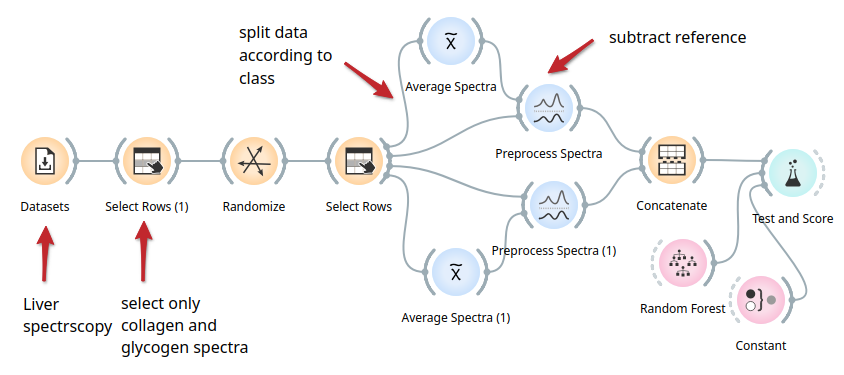
\includegraphics[scale=0.5]{different-classes-collagen.png}
  }
%\caption{Try changing the parameters!}
\end{figure*}


\section{Selection of promising features (wavenumbers) on the whole data set}

This common error in supervised modelling does not influence spectral data that much due to auto-correlation. While the influence can still be observed on small spectral data sets, let us use a gene microarray data ``Breast Cancer and Docetaxel Treatment''. First, we randomize the classes to destroy any predictive value of the features. Then we use Rank to select five columns best connected with the class according to the ANOVA test.

\begin{center}
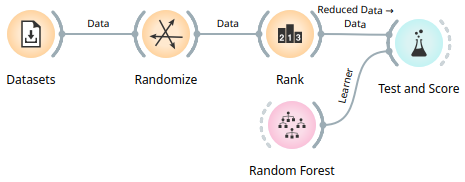
\includegraphics[scale=0.5]{column-selection.png}
\end{center}

Even though we are evaluating with cross-validation, which correctly separates training and testing sets, \widget{Test and Score} shows classification accuracy around 0.9. We had to introduce unwanted bias somewhere.

In a workflow of this size, it should not take long to find the culprit. It is the \widget{Rank} widget, or more precisely, the ANOVA test it uses to select promising features. ANOVA measures correlations between features and the class, and here lies the error: ANOVA uses information on the class before we split the data into training and testing sets. We would need to ensure that ranking is performed on the training set only to correct the error. \textbf{Verify that classes are not separable when ranking on the training set only.}


\subsection*{Exercise: repeat the same with spectral data.}

Repeat the same exercise using  spectral data. To be able to see the error there, you will need to use very few spectra. Furthermore, co-linearity in FTIR spectral data makes this difficult to see---also consider randomization that partly destroys auto-correlation.
